% Options for packages loaded elsewhere
\PassOptionsToPackage{unicode}{hyperref}
\PassOptionsToPackage{hyphens}{url}
\PassOptionsToPackage{dvipsnames,svgnames,x11names}{xcolor}
%
\documentclass[
  letterpaper,
  DIV=11,
  numbers=noendperiod]{scrartcl}

\usepackage{amsmath,amssymb}
\usepackage{lmodern}
\usepackage{iftex}
\ifPDFTeX
  \usepackage[T1]{fontenc}
  \usepackage[utf8]{inputenc}
  \usepackage{textcomp} % provide euro and other symbols
\else % if luatex or xetex
  \usepackage{unicode-math}
  \defaultfontfeatures{Scale=MatchLowercase}
  \defaultfontfeatures[\rmfamily]{Ligatures=TeX,Scale=1}
\fi
% Use upquote if available, for straight quotes in verbatim environments
\IfFileExists{upquote.sty}{\usepackage{upquote}}{}
\IfFileExists{microtype.sty}{% use microtype if available
  \usepackage[]{microtype}
  \UseMicrotypeSet[protrusion]{basicmath} % disable protrusion for tt fonts
}{}
\makeatletter
\@ifundefined{KOMAClassName}{% if non-KOMA class
  \IfFileExists{parskip.sty}{%
    \usepackage{parskip}
  }{% else
    \setlength{\parindent}{0pt}
    \setlength{\parskip}{6pt plus 2pt minus 1pt}}
}{% if KOMA class
  \KOMAoptions{parskip=half}}
\makeatother
\usepackage{xcolor}
\setlength{\emergencystretch}{3em} % prevent overfull lines
\setcounter{secnumdepth}{5}
% Make \paragraph and \subparagraph free-standing
\ifx\paragraph\undefined\else
  \let\oldparagraph\paragraph
  \renewcommand{\paragraph}[1]{\oldparagraph{#1}\mbox{}}
\fi
\ifx\subparagraph\undefined\else
  \let\oldsubparagraph\subparagraph
  \renewcommand{\subparagraph}[1]{\oldsubparagraph{#1}\mbox{}}
\fi


\providecommand{\tightlist}{%
  \setlength{\itemsep}{0pt}\setlength{\parskip}{0pt}}\usepackage{longtable,booktabs,array}
\usepackage{calc} % for calculating minipage widths
% Correct order of tables after \paragraph or \subparagraph
\usepackage{etoolbox}
\makeatletter
\patchcmd\longtable{\par}{\if@noskipsec\mbox{}\fi\par}{}{}
\makeatother
% Allow footnotes in longtable head/foot
\IfFileExists{footnotehyper.sty}{\usepackage{footnotehyper}}{\usepackage{footnote}}
\makesavenoteenv{longtable}
\usepackage{graphicx}
\makeatletter
\def\maxwidth{\ifdim\Gin@nat@width>\linewidth\linewidth\else\Gin@nat@width\fi}
\def\maxheight{\ifdim\Gin@nat@height>\textheight\textheight\else\Gin@nat@height\fi}
\makeatother
% Scale images if necessary, so that they will not overflow the page
% margins by default, and it is still possible to overwrite the defaults
% using explicit options in \includegraphics[width, height, ...]{}
\setkeys{Gin}{width=\maxwidth,height=\maxheight,keepaspectratio}
% Set default figure placement to htbp
\makeatletter
\def\fps@figure{htbp}
\makeatother

\KOMAoption{captions}{tableheading}
\makeatletter
\makeatother
\makeatletter
\makeatother
\makeatletter
\@ifpackageloaded{caption}{}{\usepackage{caption}}
\AtBeginDocument{%
\ifdefined\contentsname
  \renewcommand*\contentsname{Table of contents}
\else
  \newcommand\contentsname{Table of contents}
\fi
\ifdefined\listfigurename
  \renewcommand*\listfigurename{List of Figures}
\else
  \newcommand\listfigurename{List of Figures}
\fi
\ifdefined\listtablename
  \renewcommand*\listtablename{List of Tables}
\else
  \newcommand\listtablename{List of Tables}
\fi
\ifdefined\figurename
  \renewcommand*\figurename{Figure}
\else
  \newcommand\figurename{Figure}
\fi
\ifdefined\tablename
  \renewcommand*\tablename{Table}
\else
  \newcommand\tablename{Table}
\fi
}
\@ifpackageloaded{float}{}{\usepackage{float}}
\floatstyle{ruled}
\@ifundefined{c@chapter}{\newfloat{codelisting}{h}{lop}}{\newfloat{codelisting}{h}{lop}[chapter]}
\floatname{codelisting}{Listing}
\newcommand*\listoflistings{\listof{codelisting}{List of Listings}}
\makeatother
\makeatletter
\@ifpackageloaded{caption}{}{\usepackage{caption}}
\@ifpackageloaded{subcaption}{}{\usepackage{subcaption}}
\makeatother
\makeatletter
\@ifpackageloaded{tcolorbox}{}{\usepackage[many]{tcolorbox}}
\makeatother
\makeatletter
\@ifundefined{shadecolor}{\definecolor{shadecolor}{rgb}{.97, .97, .97}}
\makeatother
\makeatletter
\makeatother
\ifLuaTeX
  \usepackage{selnolig}  % disable illegal ligatures
\fi
\IfFileExists{bookmark.sty}{\usepackage{bookmark}}{\usepackage{hyperref}}
\IfFileExists{xurl.sty}{\usepackage{xurl}}{} % add URL line breaks if available
\urlstyle{same} % disable monospaced font for URLs
\hypersetup{
  pdftitle={Probability Theory on Finite Sets},
  pdfauthor={Michael Betancourt},
  colorlinks=true,
  linkcolor={blue},
  filecolor={Maroon},
  citecolor={Blue},
  urlcolor={Blue},
  pdfcreator={LaTeX via pandoc}}

\title{Probability Theory on Finite Sets}
\author{Michael Betancourt}
\date{January 2023}

\begin{document}
\maketitle
\ifdefined\Shaded\renewenvironment{Shaded}{\begin{tcolorbox}[frame hidden, enhanced, boxrule=0pt, interior hidden, borderline west={3pt}{0pt}{shadecolor}, breakable, sharp corners]}{\end{tcolorbox}}\fi

\renewcommand*\contentsname{Table of contents}
{
\hypersetup{linkcolor=}
\setcounter{tocdepth}{3}
\tableofcontents
}
Despite its infamous reputation the foundations of probability theory
are quite straightforward. Much of the mathematical difficulty arises
only when we implement probability theory on elaborate sets like the
real numbers, and most of the philosophical difficultly arises only when
trying to assign an interpretation to the mathematics. In this chapter I
try to avoid this baggage by introducing the basics of abstract
probability theory on the simplest, nontrivial set: a collection of a
finite number of elements.

\hypertarget{finite-sets}{%
\section{Finite Sets}\label{finite-sets}}

A \textbf{finite set} contains a finite number of distinct elements, \[
X = \{x_1, ..., x_N\}.
\] The numerical index here allows us to differentiate the between the
\(N\) individual elements but it does not necessarily imply that the
elements have any particular ordering to them. To avoid any assumption
of ordering I'll use the five element set (Figure~\ref{fig-ambient_set})
\[
X = \{\Box, \clubsuit, \diamondsuit, \heartsuit, \spadesuit\}
\] for demonstration.

\begin{figure}

{\centering 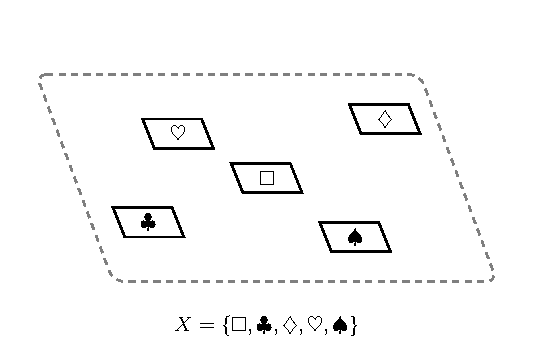
\includegraphics[width=0.5\textwidth,height=\textheight]{figures/ambient_set/ambient_set.pdf}

}

\caption{\label{fig-ambient_set}A finite set contains a finite number of
elements. This particular set contains five elements.}

\end{figure}

In practical applications of probability theory the abstract elements
\(x_{n}\) will model meaningful objects, but in this chapter I will
avoid any particular interpretation and instead focus on the
mathematical concepts. That said when \(X\) is intended to capture
\emph{all} of the objects of interest in a given application I will
refer to it as the \textbf{ambient set}.

Once we've defined an ambient set we have various ways of organizing its
individual elements and manipulating those organizations.

\hypertarget{subsets}{%
\subsection{Subsets}\label{subsets}}

A \textbf{subset} of \(X\) is any collection of elements in \(X\). To
avoid any ambiguity I will exclusively use lowercase roman letters \(x\)
to denote a variable element in the ambient set \(X\) and lowercase san
serif letters \(\mathsf{x}\) to denote a variable subset.

For example \(\mathsf{x} = \{\Box, \diamondsuit, \heartsuit\}\) is a
subset of
\(X = \{\Box, \clubsuit, \diamondsuit, \heartsuit, \spadesuit\}\)
(Figure~\ref{fig-subset}). Importantly there is no notion of
multiplicity in the concept of a subset, just membership: a subset can
include an element \(x_{n}\) but it cannot include it multiple times.

\begin{figure}

{\centering 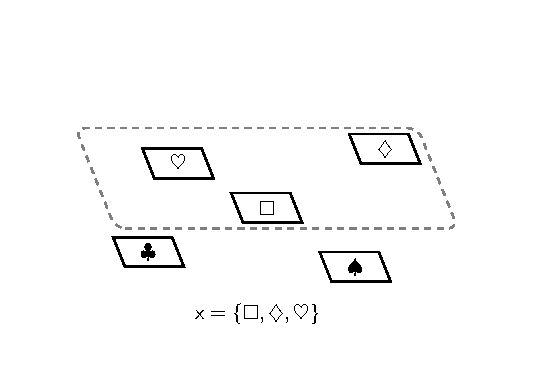
\includegraphics[width=0.5\textwidth,height=\textheight]{figures/subset/subset.pdf}

}

\caption{\label{fig-subset}A subset \(\mathsf{x} \subset X\) is any
collection of elements from the ambient set \(X\). Here
\(\mathsf{x} = \{\Box, \diamondsuit, \heartsuit\}\) contains just three
of the five elements in
\(X = \{\Box, \clubsuit, \diamondsuit, \heartsuit, \spadesuit\}\).}

\end{figure}

If \(\mathsf{x}\) is a subset of the ambient set \(X\) then we write
\(\mathsf{x} \subset X\). When \(\mathsf{x}\) might contain all of the
elements of \(X\), in which case \(\mathsf{x} = X\), then we write
\(\mathsf{x} \subseteq X\).

Subsets are \emph{recursive} objects. Selecting any elements from a
subset yields a new subset. For example the collection
\(\{\diamondsuit, \heartsuit\}\) is a subset of both the previously
introduced subset, \[
\{ \diamondsuit, \heartsuit \} \subset \{ \Box, \diamondsuit, \heartsuit \},
\] and the full ambient set, \[
\{ \diamondsuit, \heartsuit \} \subset X.
\] More formally a subset \(\mathsf{x}'\) is a subset of another subset
\(\mathsf{x}\) if and only if all of the elements in \(\mathsf{x}'\) are
also in \(\mathsf{x}\).

Regardless of how many elements a finite set \(X\) contains three
special subsets are always well-defined. The \textbf{empty set}
\(\emptyset = \{\}\) contains no elements at all. On the other hand the
entire set itself can be considered a subset containing all of the
elements. A subset containing a single element is denoted
\(\{ x_{n} \}\) and referred to as an \textbf{atomic set}.

There are \[
{N \choose n} = \frac{ N! }{ n! (N - n)!}
\] ways to select \(n\) elements from a finite set of \(N\) total
elements, and hence \({N \choose n}\) total subsets of size \(n\). For
example there is only one subset that contains no elements, \[
{N \choose 0} = \frac{ N! }{ 0! (N - 0)!} = \frac{ N! }{ N! } = 1,
\] which is just the empty set. Similarly there is only one subset that
contains all of the elements, \[
{N \choose N} = \frac{ N! }{ N! (N - N)!} = \frac{ N! }{ N! } = 1,
\] which is just the full set itself. On the other hand there are \[
{N \choose 1} = \frac{ N! }{ 1! (N - 1)!} = N
\] distinct atomics sets that contain a single element, one for each
element in \(X\).

Counting all of the subsets of all possible sizes gives \[
\sum_{n = 0}^{N} {N \choose n} = 2^{N}
\] possible subsets that we can construct from a finite set with \(N\)
elements. In other words the collection of all subsets is itself a
finite set with \(2^{N}\) elements. We refer to this set as the
\textbf{power set} of \(X\) and denote it \(2^{X}\).

When the ambient set, and all hence all of the possible elements that
any subset might contain, is fixed the prefix ``sub'' is sometimes
dropped, with all subsets simply referred to as sets. For example
collections of elements might be denoted ``sets'' when one takes the
ambient set for granted and ``subsets'' when one wants to explicitly
acknowledge the context of the ambient set. Precise terminology,
however, can vary strongly between disciplines and even individuals.

\hypertarget{subset-operations}{%
\subsection{Subset Operations}\label{subset-operations}}

We can always construct subsets element by element, but we can also
construct them by manipulating existing subsets.

For example given a subset \(\mathsf{x} \subset X\) we can construct its
\textbf{complement} by collecting all of the elements in \(X\) that are
not already in \(\mathsf{x}\). The atomic set
\(\mathsf{x} = \{ \diamondsuit \}\) contains the lone element
\(\diamondsuit\) and its complement contains the remaining elements
(Figure~\ref{fig-complement}) \[
\mathsf{x}^{c} = \{ \Box, \clubsuit, \heartsuit, \spadesuit \}.
\] By construction the complement of the empty set is the entire set,
\(\emptyset^{c} = X\), and the complement of the full set is the empty
set, \(X^{c} = \emptyset\).

\begin{figure}

{\centering 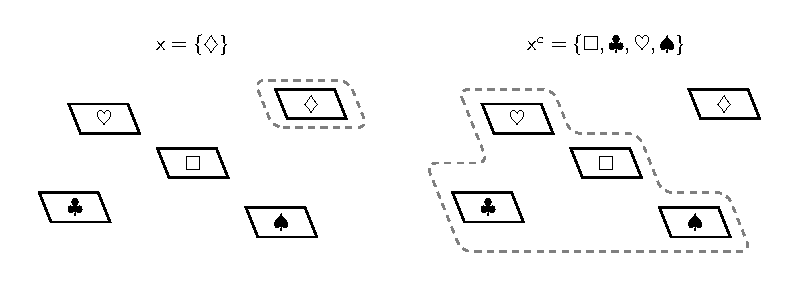
\includegraphics[width=0.75\textwidth,height=\textheight]{figures/complement/complement.pdf}

}

\caption{\label{fig-complement}The complement of a subset \(\mathsf{x}\)
is the subset \(\mathsf{x}^{c}\) consisting of all elements in the
ambient set that are not in \(\mathsf{x}\).}

\end{figure}

More formally the construction of complementary subsets defines a
\emph{unary} function that takes in a subset as input and outputs the
complementary subset, \begin{alignat*}{6}
\cdot^c :\; & 2^X & &\rightarrow& \; & 2^X &
\\
& \mathsf{x} & &\mapsto& & \mathsf{x}^{c} &.
\end{alignat*} The top line of this notation denotes the collection of
all possible inputs and outputs, here both the power set, while the
bottom line denotes the action on a particular input, here a subset
mapped into its complement. For example applying the complement operator
to the subset \(\mathsf{x} = \{ \clubsuit, \spadesuit \}\) gives \[
\mathsf{x}^{c}
= \{ \clubsuit, \spadesuit \}^{c}
= \{ \Box, \diamondsuit, \heartsuit \}.
\]

We can also construct subsets from more than one subsets. Consider, for
example, two subsets \(\mathsf{x}_1 = \{ \Box, \heartsuit \}\) and
\(\mathsf{x}_2 = \{ \Box, \spadesuit \}\) (Figure~\ref{fig-subsets}).
The collection of all elements that are contained in \emph{either}
subset is itself a subset, \[
\{ \Box, \heartsuit, \spadesuit \} \subset X,
\] as is the collection of all elements that are contained only in
\emph{both} subsets, \[
\{ \Box \} \subset X.
\] These derived subsets are referred to as the \textbf{union}, \[
\mathsf{x}_1 \cup \mathsf{x}_2
= \{ \Box, \heartsuit \} \cup \{ \Box, \spadesuit \}
= \{ \Box, \heartsuit, \spadesuit \},
\] and \textbf{intersection}, \[
\mathsf{x}_1 \cap \mathsf{x}_2
= \{ \Box, \heartsuit \} \cup \{ \Box, \spadesuit \}
= \{ \Box \},
\] respectively (Figure~\ref{fig-ui}). Note that the union and
intersection are both symmetric in the sense that either order of the
input subsets results in the same output subset, \[
\mathsf{x}_1 \cup \mathsf{x}_2 = \mathsf{x}_2 \cup \mathsf{x}_1
\] and \[
\mathsf{x}_1 \cap \mathsf{x}_2 = \mathsf{x}_2 \cap \mathsf{x}_1.
\]

\begin{figure}

{\centering 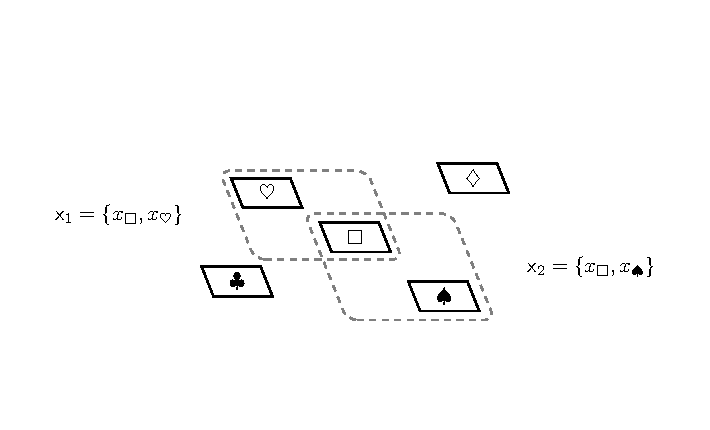
\includegraphics[width=0.75\textwidth,height=\textheight]{figures/overlapping_subsets/overlapping_subsets.pdf}

}

\caption{\label{fig-subsets}We can manipulate two subsets into a new
subset in various ways.}

\end{figure}

\begin{figure}

{\centering 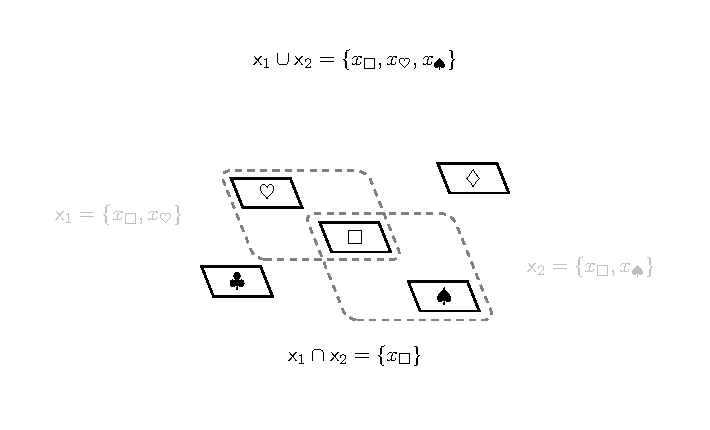
\includegraphics[width=0.75\textwidth,height=\textheight]{figures/overlapping_subsets_ui/overlapping_subsets_ui.pdf}

}

\caption{\label{fig-ui}The union of two subsets,
\(\mathsf{x}_1 \cup \mathsf{x}_2\), is a subset containing all of the
elements in either input subset. On the other hand the intersection of
two subsets, \(\mathsf{x}_1 \cap \mathsf{x}_2\), is a subset containing
just the elements that occur in both input subsets.}

\end{figure}

Two subsets are \textbf{disjoint} if they don't share any elements; in
this case their intersection is the empty set, \[
\mathsf{x}_{1} \cap \mathsf{x}_{2} = \emptyset.
\] The union and intersection of a subset with itself returns that
subset, \[
\mathsf{x} \cup \mathsf{x} = \mathsf{x} \cap \mathsf{x} = \mathsf{x}.
\] Because the empty set does not contain any elements its union with
any subset returns back that subset, \[
\mathsf{x} \cup \emptyset = \emptyset \cup \mathsf{x} = \mathsf{x},
\] and its intersection with any subset returns the empty set, \[
\mathsf{x} \cap \emptyset = \emptyset \cap \mathsf{x} = \emptyset.
\] Similarly the union of any subset with the full set returns the full
set, \[
\mathsf{x} \cup X = X \cup \mathsf{x} = X,
\] and the intersection of any subset with the full set returns back the
subset, \[
\mathsf{x} \cap X = X \cap \mathsf{x} = \mathsf{x}.
\]

Because they require two inputs the union and intersection define
\emph{binary} functions that consume \emph{two} input subsets and return
a single output subset, \begin{alignat*}{6}
\cdot \cup \cdot :\; & 2^{X} \times 2^{X}& &\rightarrow& \; & 2^{X} &
\\
& \mathsf{x}_1, \mathsf{x}_{2} & &\mapsto& & \mathsf{x}_1 \cup \mathsf{x}_2 &
\end{alignat*} and \begin{alignat*}{6}
\cdot \cap \cdot :\; & 2^{X} \times 2^{X}& &\rightarrow& \; & 2^{X} &
\\
& \mathsf{x}_1, \mathsf{x}_{2} & &\mapsto& & \mathsf{x}_1 \cap \mathsf{x}_2 &.
\end{alignat*} Here \(2^{X} \times 2^{X}\) denotes the collection of all
\emph{pairs} of subsets.

\hypertarget{measure-and-probability-over-elements}{%
\section{Measure and Probability Over
Elements}\label{measure-and-probability-over-elements}}

Measure theory, and its special case of probability theory, is often
burdened with intricate if not mysterious interpretations. From a
mathematical perspective, however, measure theory simply concerns the
consistent \textbf{allocation} of some abstract quantity across the
ambient set.

Consider a \emph{reservoir} of some positive, continuous, and
\emph{conserved} quantity, \(M \in [0, \infty]\)
(Figure~\ref{fig-reservoir}). Because \(M\) is conserved any amount
\(m_{n}\) that is allocated to the element \(x_{n} \in X\) has to be
\emph{depleted} from the reservoir, leaving less to be allocated to the
remaining elements.

We have to be careful if the total content of the reservoir \(M\) is
infinite. In this case we can allocate an infinite amount from the
reservoir while still having an infinite quantify left. At the same time
allocating an infinite amount can depleting the reservoir completely or
even leave any finite quantity. Infinity is, at the very least,
mathematically awkward.

\begin{figure}

{\centering 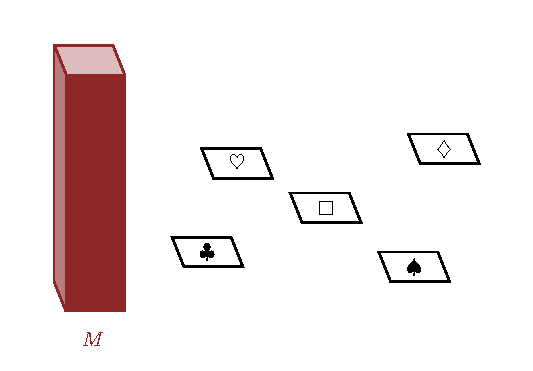
\includegraphics[width=0.5\textwidth,height=\textheight]{figures/allocations/0/0.pdf}

}

\caption{\label{fig-reservoir}Measure theory concerns the allocation of
some continuous and positive quantity \(M\) over the individual elements
of the ambient set.}

\end{figure}

To make the mathematics as useful as possible we will avoid endowing
\(M\) with any particular meaning for the time being. Instead
interpretations will arise only when we use these allocations to
\emph{model} meaningful systems.

An \emph{exhaustive} allocation of \(M\) across the ambient set ensures
that the reservoir is completely emptied. In another words all of \(M\)
has to be allocated to the elements \(x_{n} \in X\).

For example consider our demonstrative ambient set
\(X = \{\Box, \clubsuit, \diamondsuit, \heartsuit, \spadesuit \}\). If
we allocate \(m_\Box\) to \(\Box\) then that leaves \(M - m_\Box\)
remaining to allocate to the other four elements
(Figure~\ref{fig-allocationa}). Allocating \(m_\clubsuit\) to
\(\clubsuit\) depletes the reservoir a bit more
(Figure~\ref{fig-allocationb}). At the end we have to allocate all \[
M - m_{\Box} - m_{\clubsuit} - m_{\diamondsuit} - m_{\heartsuit}
\] that remains to \(\spadesuit\) to completely empty the reservoir
(Figure~\ref{fig-allocatione}).

\begin{figure}

\begin{minipage}[t]{0.50\linewidth}

{\centering 

\raisebox{-\height}{

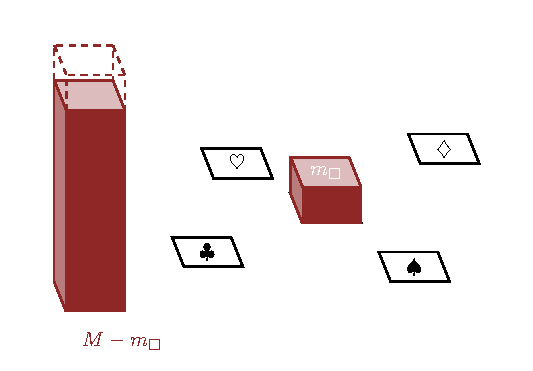
\includegraphics{figures/allocations/1/1.pdf}

}

}

\subcaption{\label{fig-allocationa}}
\end{minipage}%
%
\begin{minipage}[t]{0.50\linewidth}

{\centering 

\raisebox{-\height}{

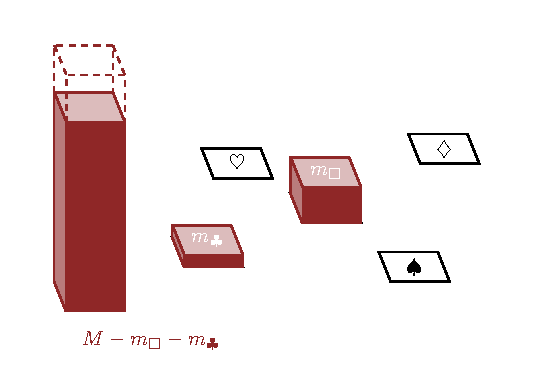
\includegraphics{figures/allocations/2/2.pdf}

}

}

\subcaption{\label{fig-allocationb}}
\end{minipage}%
\newline
\begin{minipage}[t]{0.50\linewidth}

{\centering 

\raisebox{-\height}{

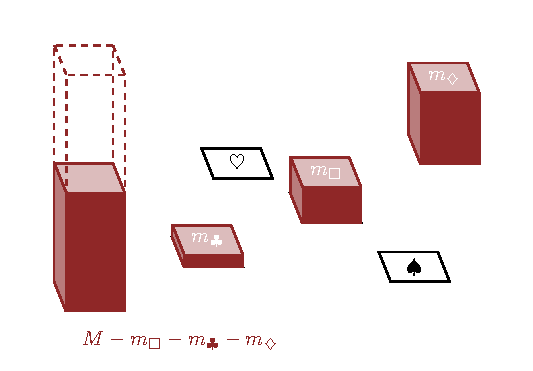
\includegraphics{figures/allocations/3/3.pdf}

}

}

\subcaption{\label{fig-allocationc}}
\end{minipage}%
%
\begin{minipage}[t]{0.50\linewidth}

{\centering 

\raisebox{-\height}{

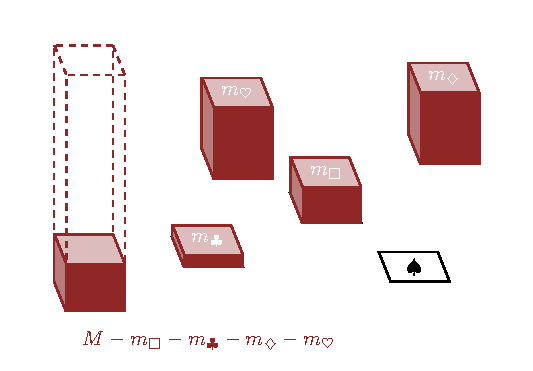
\includegraphics{figures/allocations/4/4.pdf}

}

}

\subcaption{\label{fig-allocationd}}
\end{minipage}%
\newline
\begin{minipage}[t]{0.25\linewidth}

{\centering 

~

}

\end{minipage}%
%
\begin{minipage}[t]{0.50\linewidth}

{\centering 

\raisebox{-\height}{

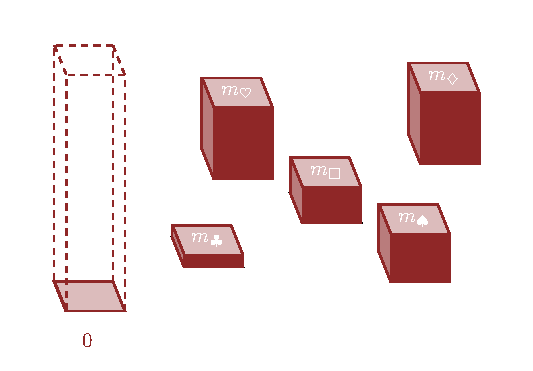
\includegraphics{figures/allocations/5/5.pdf}

}

}

\subcaption{\label{fig-allocatione}}
\end{minipage}%
%
\begin{minipage}[t]{0.25\linewidth}

{\centering 

~

}

\end{minipage}%

\caption{\label{fig-allocation}Because the total quantity \(M\) is
conserved every allocation \(m_{n}\) to an element \(x_{n} \in X\)
depletes the amount available for the allocation to the remaining
elements. An exhaustive allocation leaves nothing left in the initial
reservoir after each element has received its allocation.}

\end{figure}

A \textbf{measure} is any consistent allocation of the quantity \(M\) to
the elements of an ambient set. Mathematically any measure over a finite
set can be characterized by \(N\) numbers (Figure~\ref{fig-measure}) \[
\mu = \{ m_{1}, \ldots, m_{N} \}
\] that satisfy \[
0 \le m_{n}
\] and \[
\sum_{n = 1}^{N} m_{n} = M.
\] For example any measure over the five-element set
\(X = \{\Box, \clubsuit, \diamondsuit, \heartsuit, \spadesuit\}\) is
specified by any five positive numbers
\(\{ m_\Box, m_\clubsuit, m_\diamondsuit, m_\heartsuit, m_\spadesuit \}\)
satisfying \[
m_\Box + m_\clubsuit + m_\diamondsuit + m_\heartsuit + m_\spadesuit = M.
\]

\begin{figure}

{\centering 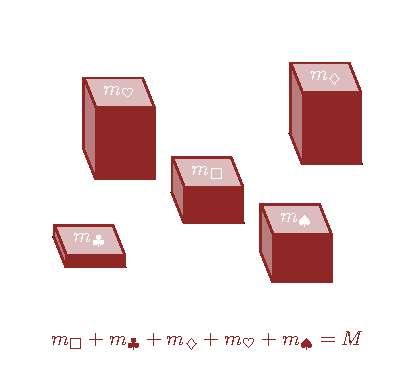
\includegraphics[width=0.5\textwidth,height=\textheight]{figures/measure/measure.pdf}

}

\caption{\label{fig-measure}A measure \(\mu\) over the finite set \(X\)
is any consistent allocation of \(M\) to the elements \(x_{n} \in X\).
Every measure can be characterized by \(N\) numbers \(m_{n}\) that sum
to \(M\), or equivalently a function that maps each element \(x_{n}\) to
its allocated measure \(m_{n}\).}

\end{figure}

The larger \(m_{n}\) the more of \(M\) is allocated to the element
\(x_{n}\). Following this terminology we will also refer to \(M\) as the
\textbf{total measure} and \(m_{n}\) as the \textbf{measure allocated to
\(x_{n}\)}.

If the total measure in infinite, \(M = \infty\), then at least one of
the elements in \(X\) \emph{has} to receive an infinite allocation in
order to empty the reservior. We can also consistently allocate infinite
measure to multiple elements, or even all of the elements, at the same
time. Infinite measures can be very generous in their allocations.

The allocation \(\{ x_{n}, m_{n} \}\) defined by a measure \(\mu\) can
also be organized into a function that maps each element to its
associated allocation, \begin{alignat*}{6}
\mu :\; & X & &\rightarrow& \; & [0, \infty] &
\\
& x_{n} & &\mapsto& & m_{n} = \mu(x_{n}) &.
\end{alignat*} A nice conceptual benefit of this functional perspective
is that instead of thinking about the global allocation
\(m_1, \ldots, m_N\) all at once we can isolate local allocations by
evaluating \(\mu\) at only a single input \(m_{n} = \mu(x_{n})\).

In general there are an infinite number of ways to allocate a total
measure to the elements of a finite set, and hence an infinite number of
measures that we can define over that set. I will denote the set of all
possible measures over \(X\) as \(\mathcal{M}(X)\).

Within this set there a few notable examples. For example a
\textbf{singular measure} allocates the total measure \(M\) to a single
element, leaving the rest with nothing
(Figure~\ref{fig-types_of_measurea}). On the other hand a
\textbf{uniform measure} allocates the same measure \(M / N\) to each
element (Figure~\ref{fig-types_of_measureb}). On finite sets there are
\(N\) distinct singular measures, one for each distinct element, and a
single unique uniform measure.

\begin{figure}

\begin{minipage}[t]{0.50\linewidth}

{\centering 

\raisebox{-\height}{

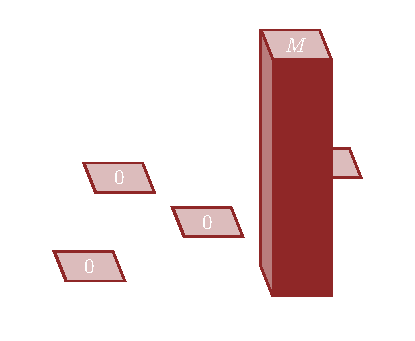
\includegraphics{figures/singular_measure/singular_measure.pdf}

}

}

\subcaption{\label{fig-types_of_measurea}}
\end{minipage}%
%
\begin{minipage}[t]{0.50\linewidth}

{\centering 

\raisebox{-\height}{

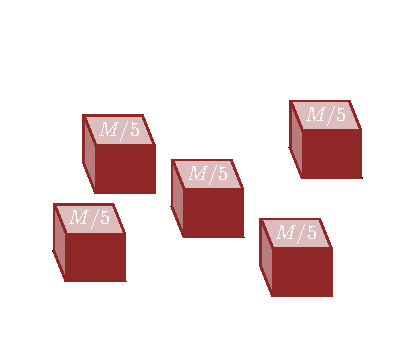
\includegraphics{figures/uniform_measure/uniform_measure.pdf}

}

}

\subcaption{\label{fig-types_of_measureb}}
\end{minipage}%

\caption{\label{fig-types_of_measure}A singular measure (a) allocates
the total measure to a single element while the uniform measure (b)
spreads the total measure to each element evenly.}

\end{figure}

Perhaps the most important class of measures, however, are measures
where the total measure is finite, \(M < \infty\). Appropriately enough
we refer to these as \textbf{finite measures}.

What makes finite measures so special is that we can always reframe the
allocation they define into a \emph{relative} one. Instead of
considering the absolute measure allocated to each element \(m_{n}\) we
can consider the \emph{proportion} of the total measure allocated to
each element, (Figure~\ref{fig-proportional}) \[
p_{n} = m_{n} / M.
\] By construction proportions are confined to the unit interval
\([0, 1]\). As with any quantity taking values in \([0, 1]\) we can
represent proportions equally well with decimals, for example
\(p_{n} = 0.2\), and percentages, \(p_{n} = 20\%\).

\begin{figure}

{\centering 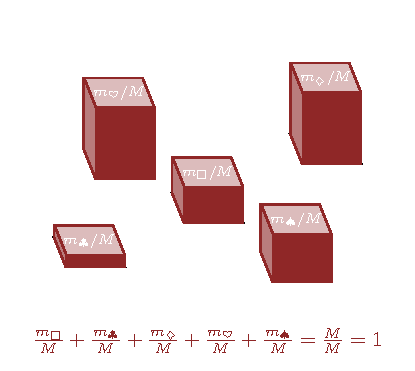
\includegraphics[width=0.5\textwidth,height=\textheight]{figures/proportional_measure/proportional_measure.pdf}

}

\caption{\label{fig-proportional}Every finite measure can be
characterized by a proportional allocation.}

\end{figure}

In other words a proportional measure defines the function
(Figure~\ref{fig-probability}) \begin{alignat*}{6}
\pi :\; & X & &\rightarrow& \; & [0, 1] &
\\
& x_{n} & &\mapsto& & p_{n} = \pi(x_{n}) &
\end{alignat*} with \[
0 \le p_{n} \le 1
\] and \[
\sum_{n = 1}^{N} p_{n} = 1.
\] A collection of variables \(\{ p_{1}, \ldots, p_{N} \}\) satisfying
these properties is referred to as a \textbf{simplex}.

\begin{figure}

{\centering 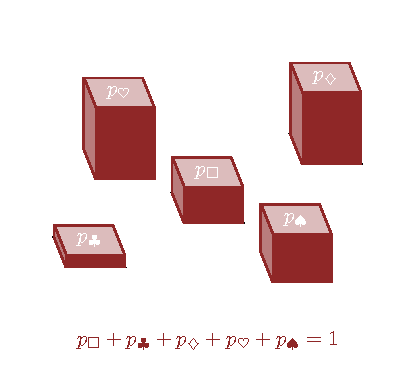
\includegraphics[width=0.5\textwidth,height=\textheight]{figures/probability_distribution/probability_distribution.pdf}

}

\caption{\label{fig-probability}A proportional allocation is also known
as a probability distribution.}

\end{figure}

More importantly a proportional measure \(\pi\) is also known as a
\textbf{probability distribution} with the proportional allocations
\(p_{n}\) denoted \textbf{probabilities}. While the term ``probability''
is often encumbered with all kinds of interpretational and philosophical
baggage its mathematical structure is really quite straightforward: on a
finite set a probability is just the proportion of some finite quantity
that is allocated to an individual element!

Philosophical tension arises only when we try to assign some meaning to
these proportional allocations. This isn't a question of mathematics but
rather \emph{applying} mathematics to model a system of interest. We'll
come back to the many different systems that can be consistently modeled
with probability theory, and hence the many different interpretations of
probability itself, in Chapter 5.

While we're on the topic of terminological issues the word
``distribution'' is not without its own problems. In mathematics the
term ``distribution'' is heavily overloaded and can be used to refer to
a variety of related but formally distinct concepts. One way to avoid
confusion is to always refer to proportional measures as ``probability
distributions'' and never just ``distributions'' alone.

\hypertarget{measure-and-probability-over-subsets}{%
\section{Measure and Probability Over
Subsets}\label{measure-and-probability-over-subsets}}

On finite sets any allocation, absolute or proportional, over the
individual elements \(x \in X\) also defines an allocation over entire
subsets \(\mathsf{x} \in 2^{X}\). The measure allocated to a subset is
just the sum of the measures allocated to the elements in that subset.
For example the measure allocated to
\(\mathsf{x} = \{ \Box, \clubsuit, \heartsuit \}\) is
\(m_{\Box} + m_{\clubsuit} + m_{\heartsuit}\)
(Figure~\ref{fig-subset_measure}).

\begin{figure}

{\centering 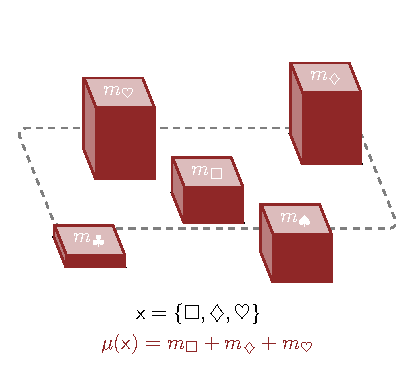
\includegraphics[width=0.5\textwidth,height=\textheight]{figures/subset_measure/subset_measure.pdf}

}

\caption{\label{fig-subset_measure}On a finite set an allocation over
individual elements also defines an allocation over any subset.}

\end{figure}

In other words a measure over individual elements
\(\mu : X \rightarrow [0, \infty]\) implicitly defines a measure over
subsets \(\mu : 2^{X} \rightarrow [0, \infty]\). Similarly a probability
distribution over individual elements \(\pi : X \rightarrow [0, 1]\)
implicitly defines a probability distribution over subsets
\(\pi : 2^{X} \rightarrow [0, 1]\).

Note that we have made the cardinal sin of \emph{overloading} our
notation so that \(\mu\) refers to both types of measures, and the only
way to differentiate them is through their different inputs; \(\mu(x)\)
denotes the element-wise measure allocated to \(x \in X\) and
\(\mu( \mathsf{x} )\) denotes the subset-wise measure allocated to
\(\mathsf{x} \in 2^X\). Maintaining different typographical conventions
for elements and subsets is critical to avoid any confusion when
overloading notation like this.

By construction any subset measure and probability distribution satisfy
a wealth of useful properties. For example for any measure \[
\mu( \emptyset ) = 0
\] and \[
\mu( X ) = \sum_{n = 1}^{N} \mu(x_{n}) = M,
\] while for any probability distribution we have
\(\pi( \emptyset ) = 0\) and \(\pi( X ) = 1\).

Even better the subset allocations play well with the subset operations.
Consider for example the two disjoint subsets
\(\mathsf{x}_{1} = \{ \Box, \diamondsuit \}\) and
\(\mathsf{x}_{2} = \{ \clubsuit, \spadesuit \}\). Because the two
subsets are disjoint their union simply combines all of their elements,
\[
\mathsf{x}_{1} \cup \mathsf{x}_{2}
=
\{ \Box, \diamondsuit \} \cup \{ \clubsuit, \spadesuit \}
=
\{ \Box, \clubsuit, \diamondsuit, \spadesuit \},
\] and the measure of that union is just the sum of the measures of the
input subsets, \begin{align*}
\mu ( \mathsf{x}_{1} \cup \mathsf{x}_{2} )
&=
\mu ( \{ \Box, \clubsuit, \diamondsuit, \spadesuit \} )
\\
&=
m_{\Box} + m_{\clubsuit} + m_{\diamondsuit} + m_{\spadesuit}
\\
&=
( m_{\Box} + m_{\diamondsuit} ) + ( m_{\clubsuit} + m_{\spadesuit} )
\\
&=
\mu( \mathsf{x}_{1} ) + \mu( \mathsf{x}_{2} ).
\end{align*}

More generally for any collection of subsets \[
\mathsf{x}_{1}, \ldots, \mathsf{x}_{K}
\] that are mutually disjoint, \[
\mathsf{x}_{k} \cap \mathsf{x}_{k'} = \emptyset
\] for \(k \ne k'\), we have \[
\mu ( \cup_{k = 1}^{K} \mathsf{x}_{k} )
=
\sum_{k = 1}^{K} \mu ( \mathsf{x}_{k} ).
\] In words if we can decompose a subset into a disjoint collection of
smaller subsets then we can also decompose the measure allocated to that
initial subset into measures allocated to the component subsets. This
consistency property is known as \textbf{additivity}.

A subset \(\mathsf{x}\) and its complement \(\mathsf{x}^{c}\) always
disjoint, \(\mathsf{x} \cap \mathsf{x}^{c} = \emptyset\). At the same
time their union covers the entire set,
\(\mathsf{x} \cup \mathsf{x}^{c} = X\). Consequently additivity implies
that \begin{align*}
M
&=
\mu (X)
\\
&=
\mu ( \mathsf{x} \cup \mathsf{x}^{c} )
\\
&= \mu ( \mathsf{x} ) + \mu ( \mathsf{x}^{c} ),
\end{align*} or \[
\mu ( \mathsf{x}^{c} ) = M - \mu ( \mathsf{x} ).
\] In words the measure allocated to the complement of a subset is the
total measure less the measure allocated to that subset. For probability
distributions this becomes even cleaner, \[
\pi ( \mathsf{x}^{c} ) = 1 - \pi ( \mathsf{x} ).
\]

When two subsets overlap we have to take into consideration that the sum
of their measures \(\mu ( \mathsf{x}_{1} ) + \mu ( \mathsf{x}_{2} )\)
double counts the allocations to any elements shared between them. For
example if \(\mathsf{x}_{1} = \{ \Box, \heartsuit \}\) and
\(\mathsf{x}_{2} = \{ \Box, \spadesuit \}\) then the union includes the
overlapping element \(\Box\) only once, \[
\mathsf{x}_{1} \cup \mathsf{x}_{2}
=
\{ \Box, \heartsuit \} \cup \{ \Box, \spadesuit \}
=
\{ \Box, \heartsuit, \spadesuit \}.
\] Consequently \begin{align*}
\mu( \mathsf{x}_{1} \cup \mathsf{x}_{2} )
&=
\mu( \{ \Box, \heartsuit, \spadesuit \} )
\\
&=
m_{\Box} + m_{\heartsuit} + m_{\spadesuit}.
\end{align*} Adding the measures allocated to the two subsets
individually, however, gives \begin{align*}
\mu( \mathsf{x}_{1} ) + \mu ( \mathsf{x}_{2} )
&=
(m_{\Box} + m_{\heartsuit} ) + ( m_{\Box} + m_{\spadesuit} )
\\
&=
m_{\Box} + m_{\Box} + m_{\heartsuit} + m_{\spadesuit}
\\
&=
m_{\Box} + \mu( \mathsf{x}_{1} \cup \mathsf{x}_{2} ).
\end{align*}

The element that is double counted here, however, is exactly the lone
element in the intersection of the two subsets
(Figure~\ref{fig-overlapping_subsets_measures}), \[
m_{\Box} = \mu( \{ \Box \} ) = \mu( \mathsf{x}_{1} \cap \mathsf{x}_{2} ).
\] In other words we can write \[
\mu( \mathsf{x}_{1} ) + \mu ( \mathsf{x}_{2} )
=
  \mu( \mathsf{x}_{1} \cap \mathsf{x}_{2} )
+ \mu( \mathsf{x}_{1} \cup \mathsf{x}_{2} ).
\] This relationship is quite general and holds for \emph{any} two
subsets regardless of their overlap.

\begin{figure}

{\centering 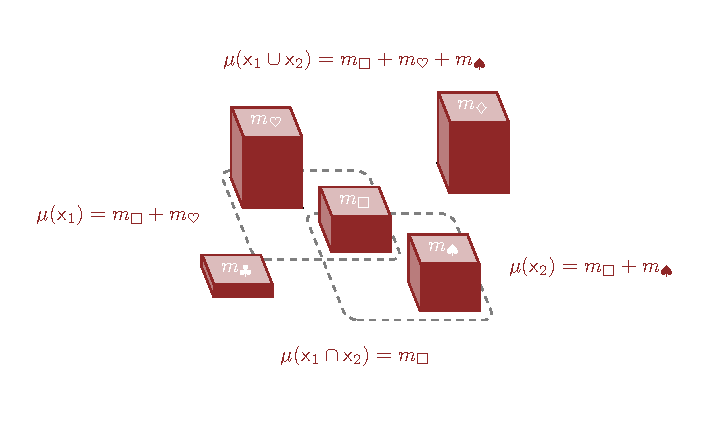
\includegraphics[width=0.75\textwidth,height=\textheight]{figures/overlapping_subsets_measures/overlapping_subsets_measures.pdf}

}

\caption{\label{fig-overlapping_subsets_measures}When two subsets
overlap the measure allocated to each double counts the measure
allocated to any overlapping elements, here \(\Box\), but the measure
allocated to their union does not. This results in an important
relationship between the measures allocated to the two subsets, the
measure allocated to their union, and the measure allocated to their
intersection.}

\end{figure}

These subset properties allow us to build up a given measure in many
different ways, each of which can useful in different circumstances.
This provides convenient flexibility when trying to apply measure theory
and probability theory in practice.

For example we can always specify a measure \emph{globally} by
specifying the individual allocations at the same time
(Figure~\ref{fig-all_at_once}). Alternatively we can specify the
allocation \emph{locally} by allocating measure to each element one at a
time (Figure~\ref{fig-one_at_a_time}).

\begin{figure}

{\centering 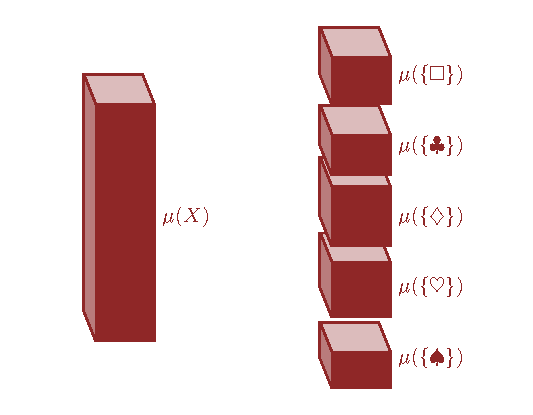
\includegraphics[width=0.33\textwidth,height=\textheight]{figures/decompositions/all_at_once/all_at_once.pdf}

}

\caption{\label{fig-all_at_once}Measures can be constructed by
specifying the individual element allocations all at once.}

\end{figure}

\begin{figure}

{\centering 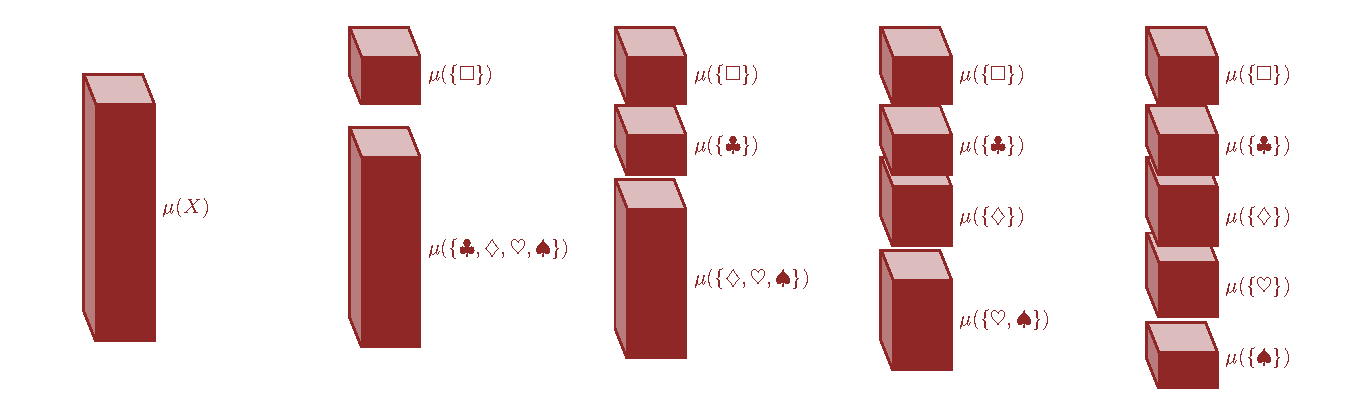
\includegraphics[width=1\textwidth,height=\textheight]{figures/decompositions/one_at_a_time/one_at_a_time.pdf}

}

\caption{\label{fig-one_at_a_time}At the same time measures can be
constructed by specifying the individual element allocations one by
one.}

\end{figure}

Critically we do not always need to start with individual allocations.
Instead we can always start by allocating the total measure to disjoint
subsets and then iteratively \emph{refining} that allocation to smaller
and smaller subsets until we reach the individual elements
(Figure~\ref{fig-refinement}).

\begin{figure}

{\centering 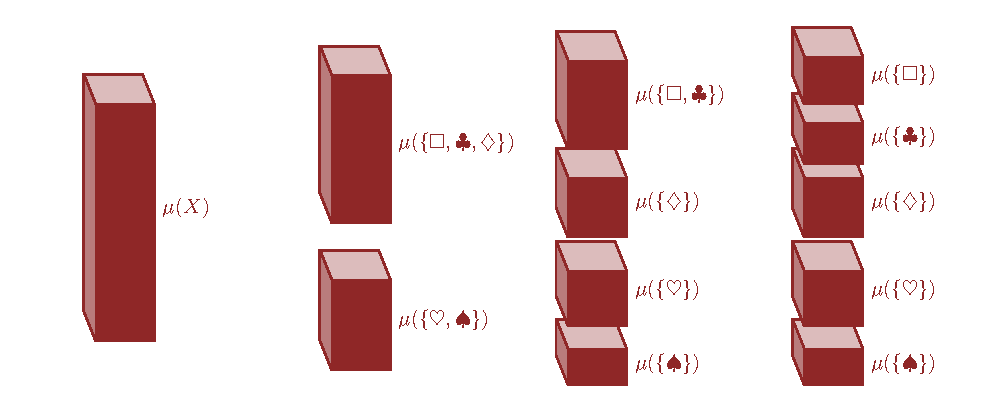
\includegraphics[width=1\textwidth,height=\textheight]{figures/decompositions/refinement/refinement.pdf}

}

\caption{\label{fig-refinement}Measures can also be constructed by
allocating the total measure to disjoint subsets and then iteratively
refining that allocation to smaller and smaller subsets.}

\end{figure}

In addition to providing flexible constructions the subset definition of
a measure \(\mu : 2^{X} \rightarrow [0, \infty]\) is also critical for
generalizing measure theory beyond finite sets. Specifically it becomes
\emph{necessary} when trying to consistently define measures on more
mathematically complicated sets like the real line. This will be the
topic of Chapter 3.

\hypertarget{acknowledgements}{%
\section{Acknowledgements}\label{acknowledgements}}

I thank Simon Duane and Edgar Merkle for helpful comments.

A very special thanks to everyone supporting me on Patreon: Aapeli
Nevala, Adam Bartonicek, Adam Fleischhacker, Adan, Adriano Yoshino, Alan
Chang, Alessandro Varacca, Alexander Bartik, Alexander Noll, Alexander
Rosteck, Anders Valind, Andrea Serafino, Andrew Mascioli, Andrew
Rouillard, Andrew Vigotsky, Angie\_Hyunji Moon, Ara Winter, asif zubair,
Austin Rochford, Austin Rochford, Avraham Adler, Ben Matthews, Ben
Swallow, Brynjolfur Gauti Jónsson, Cameron Smith, Canaan Breiss, Cat
Shark, Charles Naylor, Chase Dwelle, Chris Zawora, Christopher
Mehrvarzi, Chuck Carlson, Colin Carroll, Colin McAuliffe, Cruz, Damien
Mannion, Damon Bayer, dan mackinlay, Dan Muck, Dan W Joyce, Dan Waxman,
Dan Weitzenfeld, Daniel, Daniel Edward Marthaler, Daniel Rowe, Darshan
Pandit, Darthmaluus , David Burdelski, David Galley, David Humeau, David
Wurtz, dilsher singh dhillon, Doug Rivers, Dr.~Jobo, Dr.~Omri Har
Shemesh, Ed Cashin, Ed Henry, Edgar Merkle, edith darin, Eric LaMotte,
Erik Banek, Ero Carrera, Eugene O'Friel, Evan Cater, Fabio Pereira,
Fabio Zottele, Felipe González, Fergus Chadwick, Finn Lindgren, Florian
Wellmann, Francesco Corona, Geoff Rollins, George Ho, Granville
Matheson, Greg Sutcliffe, Guido Biele, Hamed Bastan-Hagh, Haonan Zhu,
Hector Munoz, Henri Wallen, Hugo Botha, Huib Meulenbelt, Håkan
Johansson, Ian Costley, Ian Koller, idontgetoutmuch, Ignacio Vera,
Ilaria Prosdocimi, Isaac S, Isaac Vock, J, J Michael Burgess, Jair
Andrade, James Hodgson, James McInerney, James Wade, Janek Berger, Jason
Martin, Jason Pekos, Jeff Burnett, Jeff Dotson, Jeff Helzner, Jeffrey
Burnett, Jeffrey Erlich, Jesse Wolfhagen, Jessica Graves, Joe Wagner,
John Flournoy, Jon , Jonathan H. Morgan, Jonathan St-onge, Jonathon
Vallejo, Joran Jongerling, Joseph Despres, Josh Weinstock, Joshua
Duncan, Joshua Griffith, Josué Mendoza, JU, Justin Bois, Karim Naguib,
Karim Osman, Keith O'Rourke, Kejia Shi, Kevin Foley, Kristian Gårdhus
Wichmann, Kádár András, lizzie , LOU ODETTE, Luiz Pessoa, Marc Dotson,
Marc Trunjer Kusk Nielsen, Marcel Lüthi, Marek Kwiatkowski, Mark
Donoghoe, Mark Worrall, Markus P., Martin Modrák, Matt Moores, Matthew,
Matthew Kay, Matthieu LEROY, Maurits van der Meer, Merlin Noel
Heidemanns, Michael Colaresi, Michael DeWitt, Michael Dillon, Michael
Lerner, Mick Cooney, Márton Vaitkus, N Sanders, Name, Nathaniel Burbank,
Nic Fishman, Nicholas Clark, Nicholas Cowie, Nick S, Nicolas Frisby,
Octavio Medina, Ole Rogeberg, Oliver Crook, Olivier Ma, Pablo León
Villagrá, Palwasha Khan, Patrick Kelley, Patrick Boehnke, Pau Pereira
Batlle, Peter Smits, Pieter van den Berg , ptr, Putra Manggala, Ramiro
Barrantes Reynolds, Ravin Kumar, Raúl Peralta Lozada, Riccardo Fusaroli,
Richard Nerland, Robert Frost, Robert Goldman, Robert kohn, Robert
Mitchell V, Robin Taylor, Rong Lu, Ross McCullough, Ryan Grossman, Rémi
, S Hong, Sam Levy, Scott Block, Scott Brown, Sean Pinkney, Sean Wilson,
Serena, Seth Axen, shira, Simon Duane, Simon Lilburn, Srivatsa Srinath,
sssz, Stan\_user, Stefan, Stephanie Fitzgerald, Stephen Lienhard, Steve
Bertolani, Stone Chen, Sus, Susan Holmes, Svilup, Sören Berg, Tagir
Akhmetshin, Tao Ye, Tate Tunstall, Tatsuo Okubo, Teresa Ortiz, Thiago de
Paula Oliveira, Thomas Lees, Thomas Vladeck, Tiago Cabaço, Tim Radtke,
Tom McEwen, Tomáš Frýda, Tony Wuersch, Virginia Fisher, Vitaly Druker,
Vladimir Markov, Wil Yegelwel, Will Farr, Will Kurt, Will Tudor-Evans,
woejozney, yolhaj , yureq , Zach A, Zad Rafi, and Zhengchen Cai.

\hypertarget{license}{%
\section*{License}\label{license}}
\addcontentsline{toc}{section}{License}

A repository containing all of the files used to generate this chapter
is available on
\href{https://github.com/betanalpha/quarto_chapters/tree/main/1_probability_on_finite_sets}{GitHub}.

The text and figures in this chapter are copyrighted by Michael
Betancourt and licensed under the CC BY-NC 4.0 license:

https://creativecommons.org/licenses/by-nc/4.0/



\end{document}
